\chapter{移动网络中主播端传输优化方案设计}

基于上一章的测量实验和对问题的本质分析,我们重新思考使用RTMP协议作为主播端协议的方案设计,尝试从三个不同的层面来定制化这个协议。首先,我们需要选择出一个合适的关键帧间隔,以减少视频帧之间的依赖性,从而避免应用层放大效应的发生。然后,我们尝试去优化GoP内部的丢帧策略,去尽可能多的避免丢帧,前面两个解决思路组合起来应对短时间的带宽降低。最后,我们设计了一个GoP粒度的码率自适应算法,来缓解长期的带宽衰落所带来视频质量的下降。

\section{优化空间}
\label{sec:design_space}

丢帧问题的存在明显地降低了观众的用户体验质量,应用层的丢帧放大效应加剧了,为了缓解上述问题,我们首先尝试了一些简单直接的方案,比如增加视频队列的长度,缩小GoP的时间长度。从理论上来说,这两个方案都可以减少丢帧现象的发生。因为我们知道帧之间的依赖性由于H264的视频压缩算法导致,非关键帧都是由关键帧计算得来。关键帧之间是相互独立的,依赖性只存在在一个GoP内部。通过减少关键帧间隔,我们可以减少视频帧之间的依赖性,从而减少丢帧。举个最极端的例子,如果关键帧间隔为1帧,那么帧之间完全不存在依赖性。另外,假设在关键帧为8秒的情况下,如果在一个GoP开始时,发生了一个2秒的网络抖动,那么整个GoP都会被丢弃;但是如果8秒的关键帧间隔被修改为2秒,就只会丢弃一个2秒的GoP。丢帧现象发生的另外一个原因是待发送的视频帧数据量超出队列最大容量的限制导致溢出,那么如果我们增加视频帧队列的长度,队列溢出的阈值被相应的提高,一定程度上可以减少一些视频丢帧。

为了验证上述提出的两种方案是否切实有效,并为我们的解决方案提供优化方向,我们对两种方案做一个初步的验证。

\begin{figure}[h]% use float package if you want it here
  \centering
  \begin{subfigure}{0.49\textwidth}
      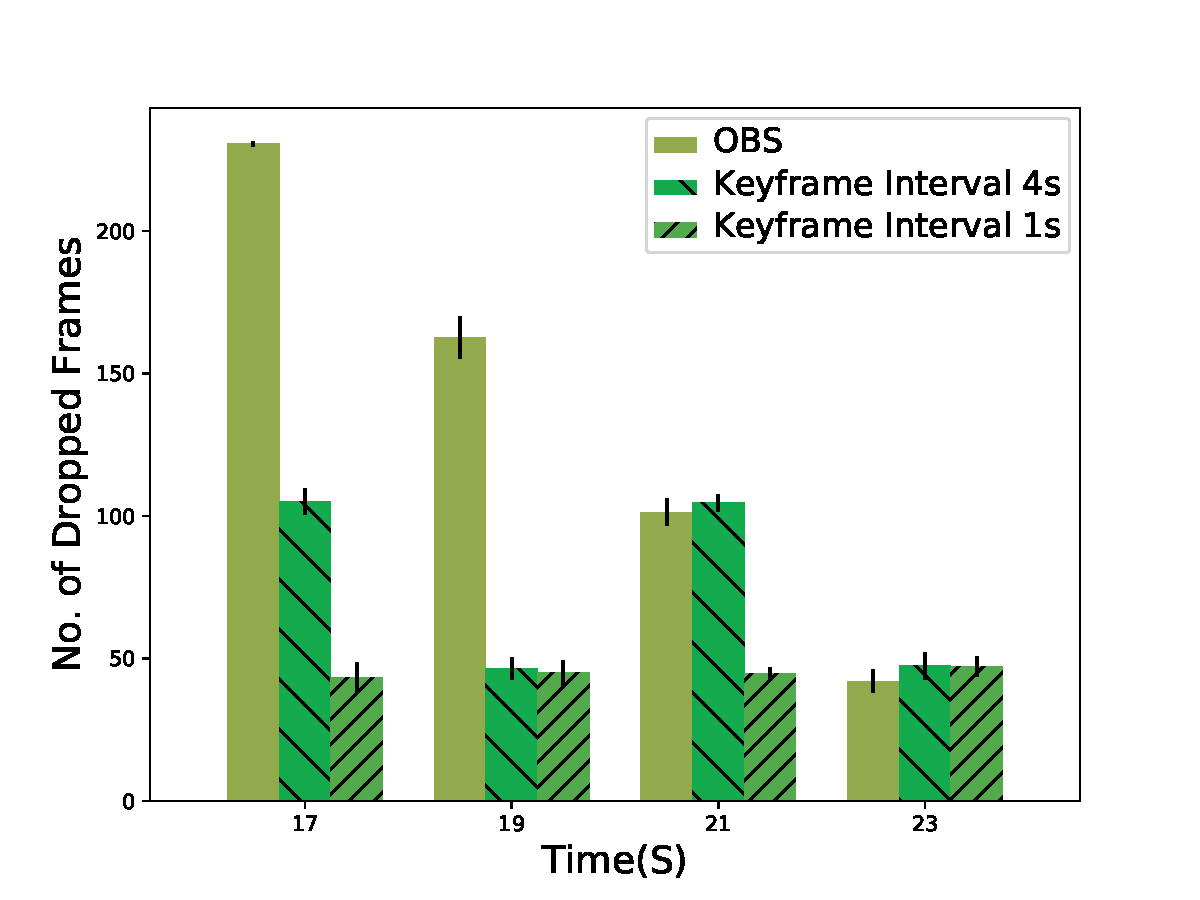
\includegraphics[width=\textwidth]{eval_IframeInterval_drop}
      \caption{不同关键帧间隔下的丢帧数}
      \label{fig:keyframe_drop}
  \end{subfigure}
  \hfill
  \begin{subfigure}{0.49\textwidth}
      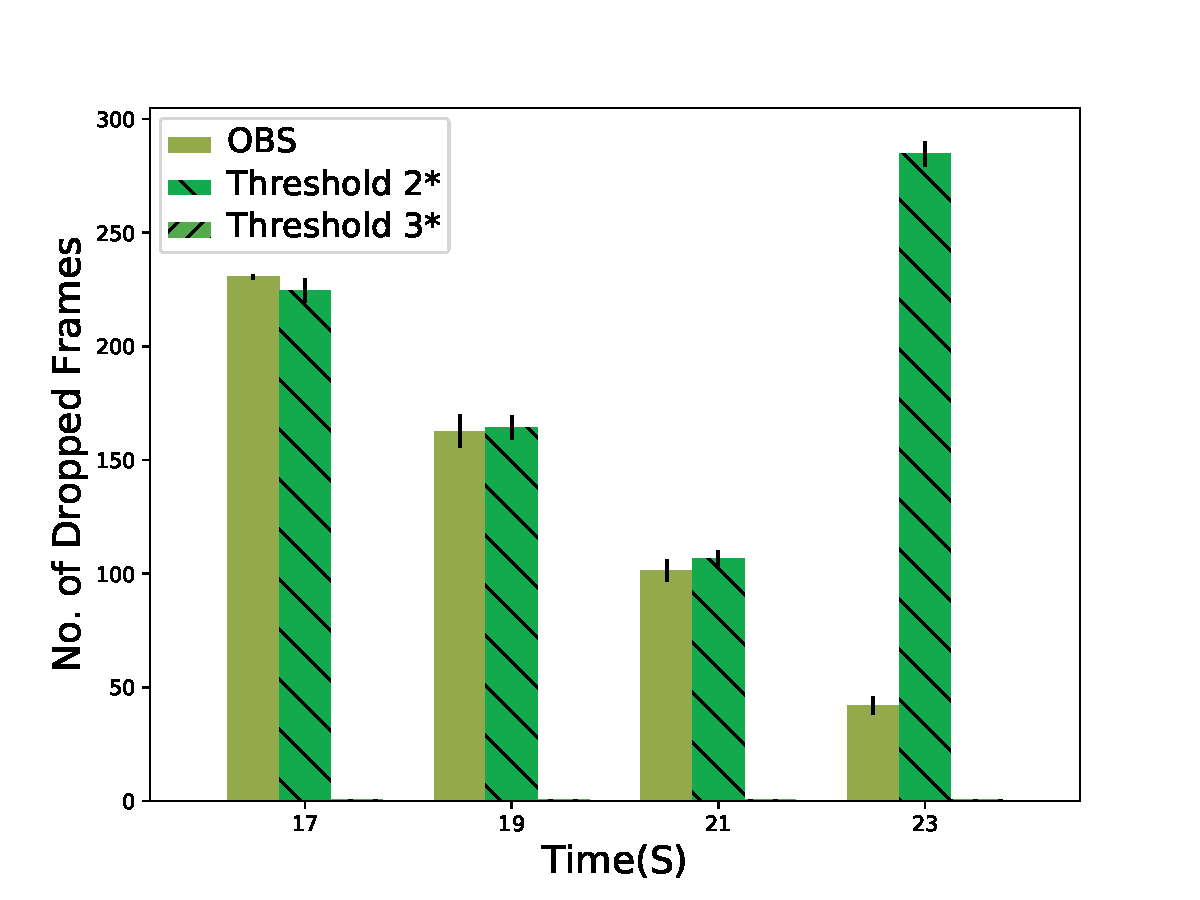
\includegraphics[width=\textwidth]{eval_threshold_drop}
      \caption{不同视频帧队列长度时的丢帧数}
      \label{fig:threshold_drop}
  \end{subfigure}
  \vspace{0.1in}
  \caption{不同编码参数下的丢帧数}
  \label{fig:prelimary_drop}
\end{figure}

\textbf{减少关键帧间隔} OBS直播软件关键帧间隔的默认值是8秒,实验中我们把关键帧间隔分别改为4秒和1秒。每次实验,我们均用OBS主播端去推流,同时为了控制变量,防止引入不必要的参数,OBS主播端推流时上传的是同一段视频。我们把OBS启动的时间定义为时间零点,为了观察关键帧对于丢帧的影响,我们分别在时间为17秒,19秒,21秒和23秒的时候断开网络连接,断开时长为2秒。丢帧的结果图展示在图~\ref{fig:keyframe_drop}中。我们可以看到,对于关键帧间隔相同的实验组来说,网络断开的时间位于一组GOP越早的时间处,丢弃的帧数则会越多。因为如果是GOP组中较早的帧,会有更多依赖于它的帧。对于默认为8秒的关键帧间隔,当断开时间分别是17秒,19秒,21秒和23秒时,丢帧数分别为238,164,105和48。因为对于关键帧间隔为8秒的情况,一个GoP的时间为16到24秒之间,17秒位于一个GoP的第1秒处,23秒的帧位于一个GoP的结尾1秒处,观察到的丢帧数也依次递增,验证了之前的理论猜想。

另外,对比在17秒时网络断开的实验组,我们发现关键帧间隔越小丢帧数减少地越明显,比如,当关键帧从8秒变到4秒再变到1秒时,丢帧数从238减到102,最后减少到46。但对于在23秒断开网络连接的实验组来说,丢帧数减少的效果并不明显。这是因为23秒处的帧在三组实验中均接近于GOP的尾部,都只有1秒时间的帧依赖于23秒处的帧。

\textbf{增加视频队列长度} OBS直播软件中默认的队列长度为P帧0.9秒,B帧0.7秒,实验中我们尝试把队列长度分别增加为原来值的2倍或3倍。原来的队列长度组合为(0.7,0.9)秒,变为2倍和3倍之后,队列阈值组合分别为(1.4,1.8)秒以及(2.1,2.7)秒。和上面的实验一样,我们重复上面两组推流过程,同时记录下来每次实验的丢帧数,最后的统计结果展示在图~\ref{fig:threshold_drop}中。当队列长度增加为原来的2倍时,丢帧数并没有减少,在17秒,19秒和21秒的情况下,丢帧数基本保持不变。在23秒时断开网络,丢帧数反而呈现增加趋势。这是因为网络断开时间为2秒,在23秒时断开网络,队列里会缓存着一个GoP的最后一秒视频帧以及下一个GoP的开始1秒视频帧。而且OBS的丢帧策略是一旦发生丢帧,丢弃视频队列里的所有P帧和B帧,则丢帧行为会丢弃一整组GoP加一秒的视频。但当我们把队列长度增加为3倍时,丢帧数基本减少为零,这是因为队列长度的丢帧阈值为2.9秒,远远大于网络断开的时间2秒,丢帧数因此均为0。

\begin{figure}[h]% use float package if you want it here
  \centering
  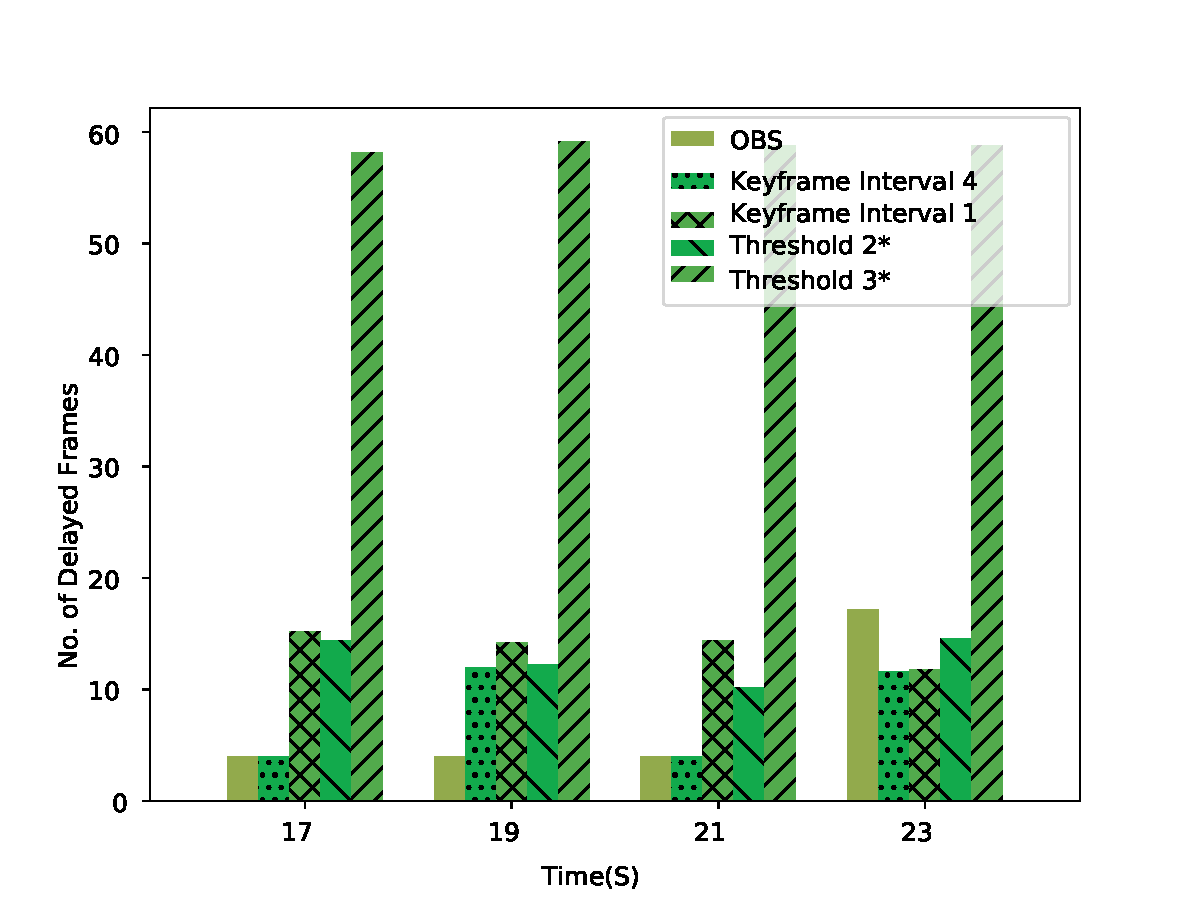
\includegraphics[width=0.7\textwidth]{timeliness}
  \caption{延迟帧的总数}
  \label{fig:timeliness}
\end{figure}

\textbf{及时性} 除了将总丢帧数作为我们的衡量指标之外,每个视频帧是否被及时的发送出去也是我们的一个重要衡量指标。为了衡量上述几组实验的及时性,我们在RTMP接收服务器处设置记录点,记录下每个视频帧的编码时间和到达时间。我们把第一个视频帧的到达时间和编码时间的差设置为0,为初始时间,记录其余视频帧和上一视频帧的编码时间和到达时间的差值,若到达时间晚于编码时间,则该视频帧被延迟了。统计总共延迟的视频帧数,并记录在图~\ref{fig:timeliness}中。从图中可以看出,当关键帧间隔变为4秒和1秒时,延迟的帧数目变化不大,维持在10帧以内,改变关键帧间隔对于及时性的影响很小。但将视频帧队列的长度增加为原来的3倍时,延迟的帧总数变为60帧左右,增加视频帧队列的长度会严重影响视频帧发送的及时性。

实验结果表明,减少关键帧间隔之后,一个短暂的网络抖动只会引起较短时间的丢帧现象,并没有进一步引起应用层的放大效应。增加视频队列的长度也可以减少丢帧的数量,因为增加视频队列的长度相当于提高了丢帧发生的阈值,减少丢帧现象的发生,自然也可以减少一部分的丢帧。

及时性指标在直播的用户体验中也占据着重要的地位,但是上面两种方案中,增加视频队列的长度违反了及时性的要求。因此,为了满足及时性的要求,我们在之后提出的解决方案中,将视频队列长度限制在足够小的数值。之后的实验中,我们将视频队列的空间大小限制为0.9秒。另外,前面的初步验证给了我们改善视频传输质量的一些方向,比如,减少关键帧间隔。结合对于丢帧根本原因的分析,我们提出通过优化视频帧产生和传输的机制去适应变化的无线网络环境,改善用户体验质量,主要包括下面几点:

\begin{enumerate}
\item \textbf{减小帧之间的依赖} 帧之间的依赖性是由于H264的视频压缩算法导致的,通过减少关键帧间隔,帧和帧之间的依赖被弱化了。然而,减少关键帧间隔会损失一定的视频质量,这个方法需要在丢帧数量和视频质量之间达到一个平衡。因为一组GoP中,一个I帧所占用的字节数很多,远远大于P帧和B帧,减少关键帧间隔,意味着同样数量的视频帧中I帧的数量增多。在同样码率的情况下,I帧数量的增多意味着每一帧分配到的数据量减少,编码器加强每一帧画面的压缩,画面的质量将会有所降低,甚至出现大的像素块。
\item \textbf{智能的丢帧策略} OBS默认的策略是当队列时间长度超出阈值后丢弃视频帧队列里所有的P帧和B帧。现在的算法设计存在一定的合理性,因为如果丢弃队列中位于队头的帧,和它处在同一个GoP中剩余的帧也就无法解码。但是如果丢弃最新的视频,老的视频帧依然存在在队列中,及时性无法保证。但是,对于队列中同时存在2个或者多个GoP的情况,一个直接的可以优化的点就是,丢弃旧的GoP的帧。这样的方法相对于OBS的默认策略会有一定的提升。设计出一个接近最优解决方案的在线的丢帧策略很重要,唯一的挑战在于帧之间存在依赖性。暴力搜索方式虽然可以找出最优解,但是由于时间复杂度太高,所以实际中并不可用。
\item \textbf{自适应码率} 图4说明了网络带宽抖动频繁发生,之前的测量显示商业平台只使用固定码率或者平均码率的方式去编码视频。平均码率的方式是指实际的带宽可以在目标码率附近波动。这两种编码方式都不能动态跟随带宽变化,当带宽下降时,会发生大量的丢帧。如果带宽降低持续时长较长的话,这种现象尤其明显。一个可能的解决方案是类似于点播情况下的DASH,在主播端动态改变码率。我们的选择是以GoP的级别去改变码率,为每一个GoP选择一个码率。引入码率自适应的方式可能会大幅度的减少丢帧。
\end{enumerate}


\section{GoP的最优选择}
如果关键帧间隔过大,当网络带宽有瞬时的降低时,会在应用层产生放大效应,丢帧数较多。但如果关键帧间隔设置的过小也会导致过高的视频压缩比,视频的清晰度会受到损害。因此,最优的GoP选择需要权衡丢帧数和视频质量两个因素。

关键帧间隔大小对于丢帧数的影响可以通过控制实验去衡量,如图~\ref{fig:keyframe_drop}所示。视频质量方面,我们用SSIM作为指标去衡量视频的清晰度~\cite{hore2010image},SSIM通过对比两幅画面的相似度去衡量视频质量。在H264编码中,SSIM旨在计算一副图片编码前后的相似性。我们重复进行多次试验,每次实验均使用同一视频,改变关键帧间隔的大小,找出SSIM在最高值$[95\%-100\%]$范围内的最小关键帧间隔。

\section{智能丢帧策略}
除了选择最优的关键帧间隔,针对短时间的网络带宽下降,一个好的丢帧策略也可以达到不错的效果。我们先假设已知全程的网络带宽,通过数学建模分析尝试找出理论上最优的丢帧策略。理论最优的算法时间复杂度较高,我们设计了一个低时间复杂度的在线算法,低时间复杂度的算法对移动设备计算能力的要求没那么高,且在实际中可以真实部署。

\subsection{丢帧策略建模}

\begin{table}[tb]
\footnotesize
\centering
\caption{丢帧策略模型所用符号表}
\label{ip_var}
{\setlength{\tabcolsep}{3pt}
\begin{tabular}{|c|c|l|}
\hline
\textbf{符号} & \textbf{类型} & \textbf{含义}                      \\ \hline
$i$               & 编号         & 帧编号                           \\ \hline
$j$               & 编号         & 时间戳编号                            \\ \hline
$x_{ij}$             & 变量      & 第j个时刻,第i帧是否在视频帧队列中\\ \hline
$y_{ij}$             & 变量      & 第j个时刻,第i帧是否已经被发送     \\ \hline
$z_{ij}$             & 变量      & 第j个时刻,第i帧是否已经被丢掉  \\ \hline
$T$               & 常量         &  总的决策时长                        \\ \hline
$T_1$             & 常量       & 一个帧能够在视频帧队列中留存的最大时长 \\ \hline
$C_j$              & 常量         & 第j个时刻的网络带宽  \\ \hline
$N$               & 常量         & 两个关键帧间的帧间隔                      \\ \hline
$S$            & 常量         & 每一帧的数据量大小                       \\ \hline
$M_{j}$       & 常量         & 第j个时刻可以发送的最大帧编号 \\ \hline
\end{tabular}}
\end{table}

首先,我们尝试计算出最优的丢帧策略可以达到的最好用户体验质量。假设每组GoP的视频帧格式已经确定,全程的网络带宽已知,一定存在一个最优的丢帧策略,在满足带宽和队列时间长度限制的情况下能够最大化观众端的体验质量。每组GoP图片组包含三种类型的帧:I帧,P帧和B帧。为了简便,建模时我们暂时忽略B帧,去研究丢帧策略的本质。所有的符号都定义在表~\ref{ip_var}中,我们将整个决策过程均匀地分为T个时隙,第i个时隙产生的帧标号为i。$x_{ij}$,$y_{ij}$,$z_{ij}$都是01变量,分别表示在第j个时刻第i个帧是否在队列中,还是已经被发送出去或者丢弃。

\textbf{帧留存性约束} 主播端每个时刻产生一个视频帧,第i个时刻新产生的帧标号为i。第i个时刻之后,第i个帧有三种去向,要么保留在视频帧队列中,要么被发送到网络中,或者被主播端丢弃。视频帧的去向可以用如下的表达式描述:
\begin{eqnarray}
% \nonumber % Remove numbering (before each equation)
  && x_{ij}+y_{ij}+z_{ij} = 0, \forall j<i \\
  && x_{ij}+y_{ij}+z_{ij} = 1, \forall j\geq i
\end{eqnarray}
如果一个视频帧已经从视频帧队列中移除,那么之后永远都不会再进入队列。同样的,一个帧被发送到网络中或者被丢弃之后,它的状态就永远变成了已发送或者被丢弃。
\begin{eqnarray}
% \nonumber % Remove numbering (before each equation)
  && x_{ij} \geq x_{i,j+1}, \forall j\geq i \\
  && y_{ij} \leq y_{i,j+1}, \forall j\geq i \\
  && z_{ij} \leq z_{i,j+1}, \forall j\geq i
\end{eqnarray}

\textbf{带宽约束} 每个时刻应该发送哪些视频帧也是减少丢帧的一个决策空间,即最优的发送策略$y_{ij}$,也是一个重要且有趣的问题。然而,我们关注于求解最优的丢帧策略,这里我们先假设主播端在满足网络容量约束的条件下,每次尽可能多的发送内容。假设每个时隙最大可发送的帧编号为$M_j$,那么第i个时刻$y_{ij}$的转移方程如下:
\begin{eqnarray}
% \nonumber % Remove numbering (before each equation)
  &&   y_{ij} = x_{i,j-1}, \forall j, i \leq M_{j}
\end{eqnarray}
等式除了满足$M_j$的约束外,可以被发送的帧必须在队列里。满足这些约束,每个时隙最大的可发送的帧编号$M_j$可以通过下面的等式来计算:
\begin{eqnarray}
% \nonumber % Remove numbering (before each equation)
 && M_j = argmax \Sigma_k x_{k,j-1} \leq C_{j}
\end{eqnarray}

\textbf{及时性约束} 一个帧在产生后的$T1$秒内必须发送出去或者被丢弃,否则就会违反了及时性约束条件。所以说,一个帧在产生的$T1$秒后,要么是被发送出去,要么就是被丢弃。
\begin{eqnarray}
% \nonumber % Remove numbering (before each equation)
  && y_{ij}+z_{ij} = 1 ,\forall j>i+T_1
\end{eqnarray}

\textbf{解码约束} 发送到网络中的帧必须要满足解码条件,否则即时视频帧成功发送到接收端也无法解码,这是对带宽资源的一种浪费,并没有充分的利用带宽。根据H264的编码准则,I帧始终可以解码,P帧只有在前面的I帧和P帧都接收到的情况下才能正常解码。
\begin{eqnarray}
% \nonumber % Remove numbering (before each equation)
  && y_{i+1,T} \geq y_{iT}, \forall i \not\equiv N-1 (\text{mod}N)
\end{eqnarray}

\textbf{优化目标} 整个问题的目标函数是去最大化传输成功的帧数。与点播视频的传输问题相比,我们的模型考虑了帧的传输及时性和是否能正常解码等约束条件,更加符合个人交互直播的场景。目标函数如下:
\begin{eqnarray}
% \nonumber % Remove numbering (before each equation)
&\min & \Sigma_i {y_{iT}} \nonumber
\label{obj}
\end{eqnarray}

\subsection{启发式算法}
分析上述目标函数和约束条件,需要求解的变量为$x_{ij}$,$y_{ij}$,$z_{ij}$,而变量的取值只有0和1两种,因此这是个整数规划问题。如果已知全程的带宽状况,可以求得该问题的离线最优解法,然而实际情况中我们并不能提前已知全部的带宽状况。另外,离线最优解法一般是通过暴力搜索去求得,该算法的时间复杂度占用资源较多,对于移动设备来说难以承受。因此,整数规划在实际情况中不可用,急需一个在线的丢帧策略。

\begin{algorithm}[htb]
\caption{GreedyDrop丢帧算法}
\label{alg:greedy-drop}
{\bf Require:} timespan:队列时间长度;dropPFrame:和P帧相关的丢帧优先级;bandwidth:每个时隙的带宽
\begin{algorithmic}[1]
\State T1 := 0.9秒, timespan :=0
\If{新产生的帧是I帧}
\State dropPFrame := False
\State \Call{入队}{视频帧队列, 新产生的帧}
\State timespan:= timespan + 1
\EndIf
\If{新产生的帧是P帧}
\If{dropPFrame or timespan $>$ T1}
\State \Call{丢弃}{新产生的帧},丢弃队列中较旧的GoP的I帧和P帧
\State timespane := timespan - 丢弃的时长
\Else
\State \Call{入队}{视频帧队列, 新产生的帧}
\State timespan := timespan + 1
\EndIf
\EndIf
\State timespan := timespan - \Call{发送的时长}{bandwidth}
\end{algorithmic}
\end{algorithm}

考虑到两个或者多个GoP同时出现在视频帧队列中的情况,我们提出了改进版的丢帧算法,GreedyDrop,如算法~\ref{alg:greedy-drop}所示。不同于默认算法将视频队列中所有的P帧都丢弃,GreedyDrop仅仅丢掉旧的GoP中的所有P帧,具体见算法的第8行描述。 因此新产生的GoP被保留了下来,在这种情况下,我们的算法至少减少了一个GoP数量的帧丢失。

\section{自适应码率}
上述的两个方案主要针对于解决短时间带宽抖动带来的应用层放大效应。为了进一步解决长时间的带宽抖动所带来的质量下降问题,我们尝试采用动态自适应码率的方式。
\subsection{动态码率建模}
不同于固定码率的算法,动态码率情况下最优的丢帧策略也不同于固定码率。因为我们的研究重点是如何动态变化码率,这里我们先采用上一节提出的丢帧策略GreedyDrop。首先,我们还是先尝试计算出通过调整码率能达到的最佳视频质量;之后,为移动设备设计一个在线可用的算法。

\begin{table}[tb]
\centering
\caption{动态码率符号表}
\label{vbr_vbr}
{\setlength{\tabcolsep}{3pt}
\begin{tabular}{|c|c|l|}
\hline
\textbf{符号} & \textbf{类型} & \textbf{含义}                      \\ \hline
$j$               & 编号         & 帧标号                            \\ \hline
$R_j$             & 变量      & 第j帧的码率 \\ \hline
$N_j$             & 变量      & 第j个时刻的GoP组数     \\ \hline
$D_j$             & 变量      & 第j个时刻的丢帧数  \\ \hline
$S_j$             & 变量   & 第j个时刻发送出的GoP组数 \\ \hline
$C_j$              & 变量         & 第j个时刻的网络带宽           \\ \hline
$T_k^j$               & 变量         & 第j时刻第k个GoP的剩余时间  \\ \hline
$R_k^j$            & 变量         & 第j个时刻第k个GoP的码率  \\ \hline
$Rest_j$       & 变量 & 第j个时刻发送剩余的GoP的时长 \\ \hline
$T$               & 变量         & 总决策时长                       \\ \hline
$T_1$               &变量          & 一个帧能够在队列中留存的时间阈值 \\
\hline\end{tabular}}
\end{table}

建模使用的符号全部包含在表~\ref{vbr_vbr}中。为了研究最优的动态码率,我们引入了一组码率相关的变量,其中$R_j$表现第j帧所对应的码率。使用GreedyDrop作为我们的丢帧策略,效益函数可以建模成下面的等式。
\begin{eqnarray}
&\max & \sum R_j- \alpha\sum|R_{j+1}-R_j|-\beta\sum D_j \nonumber
\label{vbr_obj}
\end{eqnarray}
等式中的第一项是选择的视频清晰度带来的效益,第二项代表由于视频的码率切换带来的损失,最后一项等于由于网络抖动丢帧带来的损失。变量$\alpha$和$\beta$对应码率切换损失和丢帧损失的系数。

\textbf{码率约束} 因为我们码率调整的粒度为一个GoP组,所以一个GoP内部的码率必须相同。$mod$是取余函数。
\begin{eqnarray}
% \nonumber % Remove numbering (before each equation)
  && R_{j+1}=R_j, \forall mod(j,M)\not\equiv M-1
\end{eqnarray}

\textbf{带宽约束} 在有限带宽情况下,最多能够发送的GoP组数为$S_j$,计算公式如下:
\begin{eqnarray}
% \nonumber % Remove numbering (before each equation)
  && S_j = argmax{\sum_k R_k^j*T_k^j \leq C_j}, \forall j
\end{eqnarray}

\textbf{及时性约束} 视频队列的时间长度要小于时间阈值,否则,就应该执行丢帧操作。第j个时刻帧发送出去之后,队列里剩余的时间长度为$Rest_j$,先判断剩余的时间长度$Rest_j$是否大于$T1$,如果大于$T1$的话,则丢弃最旧的一组GoP。上述行为可以用下面的等式组来表示:
\begin{eqnarray}
% \nonumber % Remove numbering (before each equation)
  && Rest_j = (C_j- \sum_{S_j} R_k^j*T_k^j)/R_{S_j+1}^j, \forall j \\
  && F_j = sgn(\sum_{S_j+1} T_k^j - Rest_j-T_1), \forall j \\
  && D_j = F_j*(T_{S_j+1}^j-Rest_j), \forall j
\end{eqnarray}
其中,$sgn$是修正版的符号函数,当变量大于0时,函数值等于1;否则函数值等于0。

\textbf{状态转移方程} 约束条件组(4-16)(4-17)(4-18)(4-19)(4-20)是队列中剩余每组GoP的码率和剩余时间的转移方程。等式(4-15)描述了第j+1个时隙的GoP组数,等式(4-15)的最后两项 $1-sg(mod(j,M))$ 取决于第j个帧是否是关键帧。
\begin{eqnarray}
% \nonumber % Remove numbering (before each equation)
  && N_{j+1}=N_j-S_j-F_j+1-sgn(mod(j,M)), \forall j \\
  && R_k^{j+1}=R_{k+S_j+F_j}^j, \forall j, k\in \{1,N_j-S_j-F_j\} \\
  && R_{N_j-S_j-F_j+1}^{j+1} = R_{j+1}, \forall mod(j,M) \equiv 0 \\
  && T_k^{j+1} = T_{k+S_j+F_j}^j, \forall j, k\in\{1, N_j-S_j-F_j\} \\
  && T_{N_j-S_j-F_j}^{j+1} = T_{N_j-S_j-F_j}^{j+1} - D_j - Rest_j , \forall j \\
  && T_{N_j-S_j-F_j+1}^{j+1}=1, \forall mod(j,M)\equiv 0
\end{eqnarray}

离线最优的解决方案很难求解。假设对于每个GoP组,主播端可以从M个码率中任意选择,那么对于T个GoP组,码率选择的计算复杂度等于$M^T$,达到了指数级复杂度。

\subsection{启发式动态码率算法}
指数级复杂度的问题很难在有限的时间内求得答案。除此之外,离线最优算法需要已知未来的全部带宽。这种长时间的带宽预测精确度很难保证,一个直接的想法是根据实时带宽改变视频的码率。视频队列中的剩余数据量大小也是选择码率的有效依据。我们提出了启发式的动态码率算法,简称GVBR,算法的伪代码如图~\ref{alg:gvbr_adaptative}所示。根据GVBR算法,在第j个时刻,主播端执行下面两个关键步骤。$\eta$是有关丢帧和码率的系数。

\begin{algorithm}[htb]
\caption{GVBR码率自适应算法}
\label{alg:gvbr_adaptative}
\begin{algorithmic}[1]
\State Rest:=0, Send:=0, Drop:=0, $\eta$
\For {$j=1$ to T}
\State 根据前面$tau$个时隙的历史带宽记录[$C_{j-tau}$,$C_{j-1}$],计算调和平均值来预估第j个时隙的带宽$C_j$
\State 选择一个最大可用码率$R_j$,小于等式$(C_j-rest)/\eta$
\State 在满足带宽约束的条件下,发送队列中的视频帧,发送的帧数为 $Send$
\State 判断是否需要丢弃额外的帧,丢帧数为 $Drop$
\State 计算视频帧队列中剩余的数据量 $Rest=Rest+R_j-Send-Drop$
\EndFor
\end{algorithmic}
\end{algorithm}

\begin{enumerate}
  \item 带宽估计 在Festive和MPC中,均用调和平均值来估计未来带宽。越精确的码率估计,我们的算法性能会越好。这篇文章中,因为我们的研究重点不是针对带宽进行预估,我们暂时采用调和平均的方式估计带宽。
  \item 码率选择 为了避免在直播过程中产生频繁的丢包,选择一个合适的码率尤为重要。假设已知未来的带宽$C_j$和队列现在的数据量大小$Rest$,我们提出的启发式算法会选择比$(C_j-Rest)/\eta$低的最高码率。
\end{enumerate}

GVBR结合了我们提出的三种策略,是一整套改善主播端传输质量的解决方案,包含GoP层面和帧层面。

\section{本章小结}
本章从三个层面提出了针对移动网络状况下主播端的传输质量优化机制,包含GoP层面和GoP内部的机制。

首先,我们通过多次重复控制实验的方法来确定最优的关键帧间隔。最优的关键帧间隔选择要同时考虑丢帧现象的发生以及视频质量的影响。

其次,本章对于移动网络状况下主播端的丢帧策略进行了理论建模,考虑视频GoP内部帧结构以及网络带宽全部已知的情况下,最优的丢帧策略。同时,考虑到移动设备的计算资源以及实际运行的情况,提出了一个在线的启发式丢帧策略,命名为GreedyDrop算法。

最后,在前两步优化的基础上,进一步优化由于长时间的网络带宽抖动带来的视频质量下降的问题。我们对移动网络状况下主播端的码率自适应算法进行了理论建模,丢帧策略和关键帧间隔采用前两步的结论。动态码率的效益函数综合考虑了每个GoP选择的码率,码率间的切换以及丢帧数等因素。为了实际可用,我们根据视频帧队列的剩余空间以及网络带宽去选择当前的码率,命名为GVBR算法。GVBR算法结合了三种算法的优势,是一整套的移动网络下主播端传输优化的解决方案。